\documentclass{jarticle}
\usepackage[dvipdfmx]{graphicx}
\usepackage{here}
\usepackage{listings,jlisting}


\lstset{
  basicstyle={\ttfamily},
  identifierstyle={\small},
  commentstyle={\smallitshape},
  keywordstyle={\small\bfseries},
  ndkeywordstyle={\small},
  stringstyle={\small\ttfamily},
  frame={tb},
  breaklines=true,
  columns=[l]{fullflexible},
  numbers=left,
  xrightmargin=0zw,
  xleftmargin=3zw,
  numberstyle={\scriptsize},
  stepnumber=1,
  numbersep=1zw,
  lineskip=-0.5ex
}

\title{{システム実験}\\基礎実験5レポート}
\author{6119019056 山口力也}
\date{2019/05/24日提出}

\begin{document}
\maketitle

\section{基礎実験第五回の概要}
基礎実験第5回目の実験の目的,実験した実験の概要,および理解した事柄を100~200字程度で説明せよ.

本実験では,Arduinoの持つ通信機能のうちシリアル通信に関する実験を行う.シリアル通信は,古くからコンピュータ間の通信に使用されてきた通信方式であり,多くのマイコンんいしリアル通信機能が搭載されている.シリアル通信を用いることで,マイコンの外部に接続されたデバイスと決められたプロトコルに従って通信を行える.以下に実験目標を示す.
\begin{itemize}
\item シリアル通信の原理を理解する.
\item シリアル通信を使いこなす.
\item マイコンとパソコン間でデータを送受信できる.
\item センサのデータをマイコン・パソコンで処理できる.
\item ディジタルI/O,AD変換,割り込みなどを統合的に扱える.

\end{itemize}

\section{復習と確認}
ブレッドボード上に回路を実装する際の注意点を説明せよ.また,C言語によるプログラムとスケッチの違いについて説明せよ.さらに,シリアルモニタ使用に関する注意点を述べよ.

汎用的な回路を同じブレッドボード上に実装することが度々あるが,関係のない回路と繋がらないように注意するべきである.また,LEDなどを実装する際はLEDと電源の間に電流制限抵抗を用いることも忘れてはならない.C言語によるプログラムとスケッチの違いについては,実装する際にある.C言語の場合実行ファイルを実行したときのみプログラムが実行されるが,スケッチの場合一度マイコンにスケッチを書き込むと電源を入れるたび書き込んだスケッチが動作する.そのため,例えば単に電源を入れただけと思っていても前回書き込んだプログラムが実行されている可能性があるので注意する必要がある.
シリアルモニタ使用に関しては,いくつか注意点がある.シリアル通信使用する際,コンピュータとのデータ転送レートを設定する必要がある.Arduinoではデフォルトで9600bpsが設定されているが,マイコン側の転送レートを変更した場合にはパソコン側のシリアルモニタの転送レート設定も同様に変更しないと正しくデータを受信できない.

\section{回路実装}
演習2.5.3において実装したブレッドボード配線図を報告せよ.

以下図\ref{fig:2-5-3bread}に実装したブレッドボード配線図を示す.


\begin{figure}[H]
\begin{center}
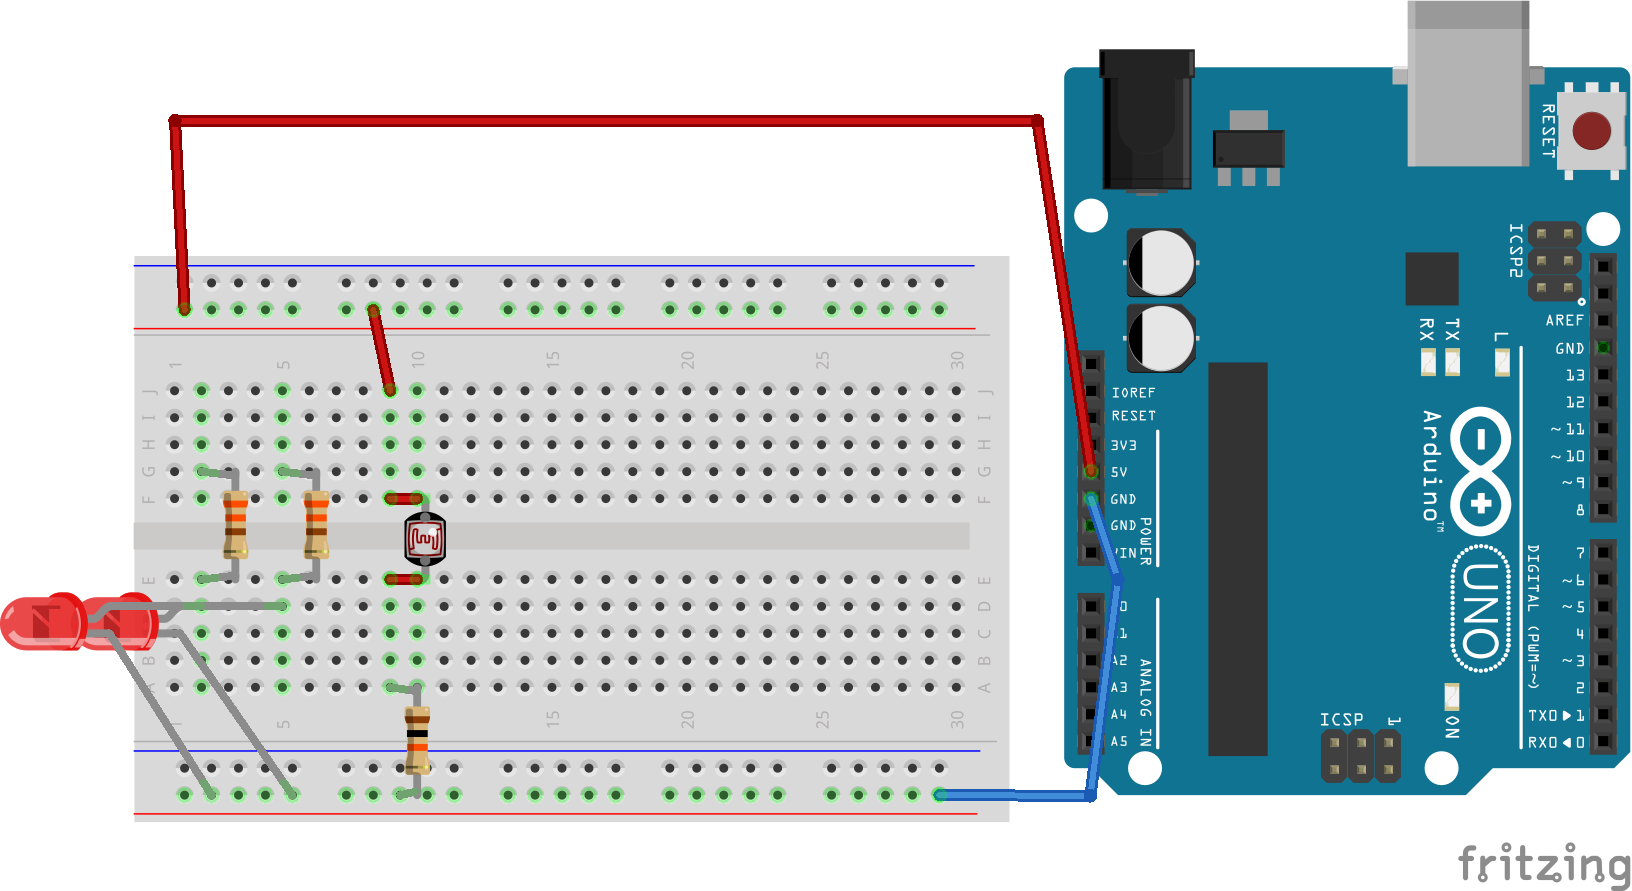
\includegraphics[width=7.0cm]{images/2-5-3bread.png}
\caption{演習2.5.3で実装した回路の配線図}
\label{fig:2-5-3bread}
\end{center}
\end{figure}

\section{マイコンの受信データに対応したLEDの状態変化およびマイコンからLEDの状態を送信}
課題2.5.1において実装したスケッチを報告せよ.また,スケッチ作成において工夫した点を記せ.さらに,マイコンが受信した文字を数字に変換して処理する方法を提案せよ.

以下ソースコード\ref{code:kadai2-5-1}に実装したスケッチを示す.
\begin{lstlisting}[caption = 課題2.5.1,label=code:kadai2-5-1][H]
const int LED_RED_PIN = 13; //LED(赤)を13番ポートに定義
const int LED_YEL_PIN = 9; //LED(黄)を9番ポートに定義
int output_red = LOW; //赤色LEDへの出力用
int output_yel = LOW;
void setup() {
  pinMode(LED_RED_PIN,OUTPUT); //赤色LEDを出力として設定
  pinMode(LED_YEL_PIN,OUTPUT); //黄色LEDを出力として設定
  Serial.begin(9600); //シリアル通信開始:転送レート9600
}

void loop() {
  if(Serial.available()>0){ //パソコンからデータを受信
    int recv = Serial.read();
    recv -= 48; //数字に変換
    Serial.println(recv);
    if(recv == 0){ //'0'の場合
      output_red = HIGH;
      output_yel = LOW;
    }
    else if(recv == 1){ //'1'の場合
      output_red = LOW;
      output_yel = HIGH;
    }
    else if(recv == -38){ //改行コードが来た時
      //何もしない
    }
    else{
      output_red = HIGH;
      output_yel = HIGH;
    }
    //Serial.println("I received!"); //パソコンへ応答を返す(送信)
    Serial.print("LED1:");
    Serial.println(output_red);
    Serial.print("LED2:");
    Serial.println(output_yel);
    digitalWrite(LED_RED_PIN,output_red); //赤色LEDの点灯・消灯
    digitalWrite(LED_YEL_PIN,output_yel); //赤色LEDの点灯・消灯
  }
}
\end{lstlisting}

工夫した点は,改行コードが来た時の対応をつくったところである.マイコンが受信した文字を数字に変換するには,ASCIIテーブルから変換する必要がある.例えばマイコンが10進数で"65"という文字を受信した場合,ASCIIテーブルから変換されて,"A"という文字になる.数字に変換したい場合はAという文字をもう一度"65"という文字に変換してやる必要がある.

\section{温度センサを用いたマイコンの温度情報のPCへの送信およびそのグラフ化}
演習2.5.6において作成したグラフを報告せよ.

以下図\ref{fig:enshu2-5-6}に作成したグラフを示す.

\begin{figure}[H]
\begin{center}
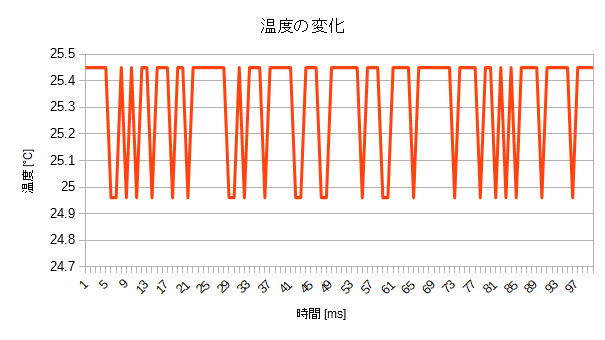
\includegraphics[width=7.0cm]{images/enshu2-5-6.png}
\caption{演習2.5.6で作成したグラフ}
\label{fig:enshu2-5-6}
\end{center}
\end{figure}

\section{millis関数によるデータ解析区間の設定,温度センサ情報のPCへの送信および温度情報グラフ化}
演習2.5.7において作成したグラフを報告せよ.

以下図\ref{fig:enshu2-5-7}に作成したグラフを示す.

\begin{figure}[H]
\begin{center}
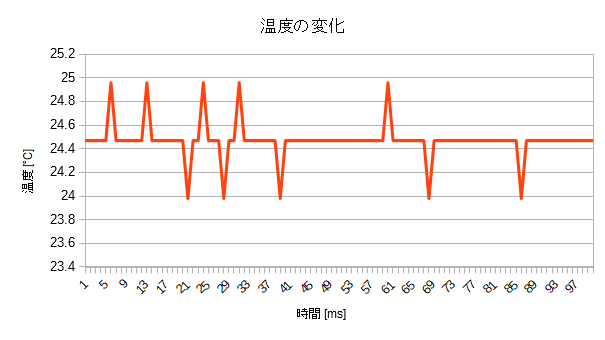
\includegraphics[width=7.0cm]{images/enshu2-5-7.png}
\caption{演習2.5.7で作成したグラフ}
\label{fig:enshu2-5-7}
\end{center}
\end{figure}

\section{温度センサを用いた解析済み温度情報のマイコンのPCへの送信およびグラフ化}
課題2.5.2で実装したスケッチおよび作成したグラフを報告せよ.また,工夫した点を記せ.演習2.5.6で作成されたグラフとの違いを説明せよ.

以下ソースコード\ref{code:kadai2-5-2}に実装したスケッチを示す.
\begin{lstlisting}[caption = 課題2.5.2,label=code:kadai2-5-2][H]
unsigned long timePrev = 0;
int count = 0;
double average = 0;
double sum= 0;
void SendData(){
  Serial.println(average);
  count++;
}
void setup() {
  Serial.begin(9600);
  Serial.println("start!");
  timePrev = millis();
}

void loop() {
  if(count < 100){
    double sum = 0; //合計格納用変数
    long int i = 0; //合計測定回数格納用変数
    while (1){//100ms経つまで
      unsigned long timeNow = millis(); //現在時間を格納
      if(timeNow - timePrev <= 100){ //100ms経つまで
        int sensorValue = analogRead(A0); //A0の値を格納
        double vo = sensorValue*(5.0/1024.0);
        double Temp = (vo*1000.0 - 600.0)/10.0;
        sum += Temp;
        i++;
      }
      else{
        timePrev = timeNow;
        break;
      }
   }
   average = sum / i;
   SendData();
  }
}
\end{lstlisting}
工夫した点は,SendDataという関数を作って,データを送る部分を分けて見やすくそして使いやすくしたところである.

また,以下図\ref{fig:kadai2-5-2}に作成したグラフを示す.

\begin{figure}[H]
\begin{center}
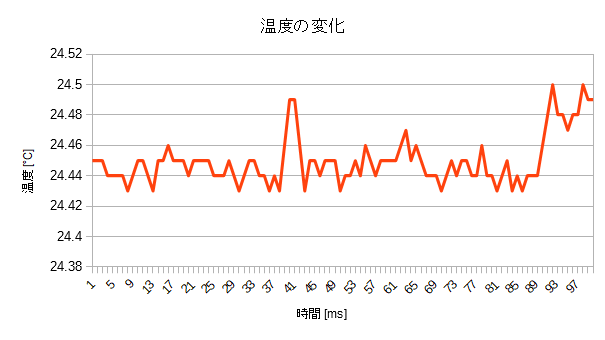
\includegraphics[width=7.0cm]{images/kadai2-5-2.png}
\caption{課題2.5.2で作成したグラフ}
\label{fig:kadai2-5-2}
\end{center}
\end{figure}

演習2.5.6で作成された図\ref{fig:enshu2-5-6}との違いは,データ解析区間を作ることでグラフが滑らかになっていることである.平均値を取らずに,グラフを作ると何らかの影響で飛び出た値が出た時に,そのままその値を出力してしまうためがたがたのグラフになってしまう

\section{照度センサによるマイコンからPCヘの解析済み温度情報の送信,グラフ化および解析結果に対応したLEDの発光}
課題2.5.3で実装したスケッチおよび作成したグラフを報告せよ.また,工夫した点を記せ.さらに,データ解析(区間平均の算出)の必要性について考察せよ.

以下ソースコード\ref{code:kadai2-5-3}に実装したスケッチを示す.
\begin{lstlisting}[caption = 課題2.5.3,label=code:kadai2-5-3][H]
unsigned long timePrev = 0;
int count = 0;
double average = 0;
double sum = 0;
int output = 0;
const int LED_PIN = 9; //9番ポートをLEDに設定
void SendData(){
  Serial.println(average);
  count++;
}
void setup() {
  analogWrite(LED_PIN,OUTPUT);
  Serial.begin(9600);
  Serial.println("start!");
  timePrev = millis();
}

void loop() {
  if(count < 30){ //15秒経つまで(500ms×30)
    double sum = 0; //合計格納用変数
    long int i = 0; //合計測定回数格納用変数
    while (1){//500ms経つまで
      unsigned long timeNow = millis(); //現在時間を格納
      if(timeNow - timePrev <= 500){ //500ms経つまで
        int sensorValue = analogRead(A0); //A0の値を格納
        double vo = sensorValue*(5.0/1024.0);
        double L = 222*vo;
        sum += L;
        i++;
      }
      else{
        timePrev = timeNow;
        break;
      }
   }
   average = sum / i; 
   SendData();
   output = int(average*255);
   if(output > 255){
    output = 255;
   }
   analogWrite(LED_PIN,output); //照度1で255(MAX)出力
  }
}
\end{lstlisting}
工夫した点は,出力の部分で事前に照度の最大が1付近であったことを確認したのでそのあたりを最大値として,また照度が1を超えた際の処理も入れておいところである.
また,以下図\ref{fig:kadai2-5-3}に作成したグラフを示す.

\begin{figure}[H]
\begin{center}
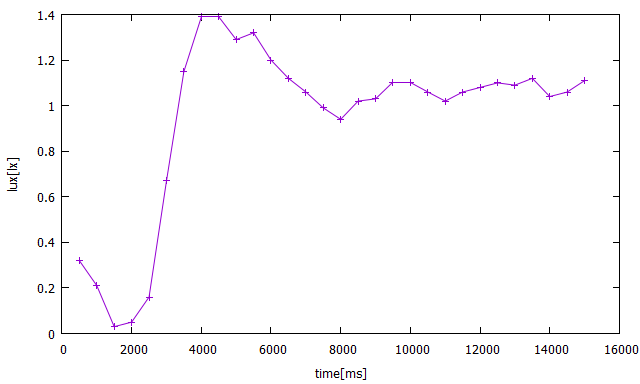
\includegraphics[width=7.0cm]{images/kadai2-5-3.png}
\caption{課題2.5.3で作成したグラフ}
\label{fig:kadai2-5-3}
\end{center}
\end{figure}

データ解析の必要性について.データ解析区間があることで比較的にまとまった値がでるので,突然変な値が何らかの理由で入ったとしても平均化されるためそこまでデータに支障がでない.そういう意味ではデータ解析区間を設けることは必要であると考えられる.


\section{発展課題2.5.1:マイコンのデータ送受信の確認}
以下ソースコード\ref{code:hatten2-5-1}に実装したスケッチを示す.

\begin{lstlisting}[caption = 発展課題2.5.1,label=code:hatten2-5-1][H]
void setup() {
  Serial.begin(9600); //転送レート9600に設定
}

void loop() {
  if(Serial.available() > 0){ //パソコンからデータを受信
    int receive = 0; //受信データ
    int birthday[4] = {0}; //表示用配列
    int kekka = 0;
    int i = 0; //配列の要素カウント用
    while(1){
      if(Serial.available() > 0){ //受信したら
        receive = Serial.read();
        if( 47 < receive && receive <58){ //受信データが数字のASCIIコードの時
          receive -= 48; //数字に変換
          birthday[i] = receive; //配列に入れる
          i++; //配列の要素をずらす
        }
        if( receive == 10){ //改行が来たら
          break; //ループを抜ける
        }
      }
    }
    birthday[2] += birthday[0]; //誕生日の2桁目に誕生月の2桁目を足す
    if (birthday[3] + birthday[1] >= 10){//もし誕生日の1桁目と誕生月の1桁目の和が10以上なら
      birthday[2]++; //繰り上げで誕生日の2桁目に1足す
      birthday[3] += birthday[1] -10; //誕生日の1桁目は足した数-10
    }
    else{ //誕生日の1桁目と誕生月の1桁目の和が10未満なら
      birthday[3] += birthday[1]; //誕生日の1桁目に誕生月の1桁目を足す
    }
    for ( i = 0; i < 4 ; i++){
      Serial.print(birthday[i]); //シリアルモニタに配列の要素を表示
    }
    Serial.println(); //改行
  }
}
\end{lstlisting}
工夫した点は,シリアルモニタから送信された文字を一度配列に格納したところである.普通にSerial.read()した場合,誕生月を誕生日に足す処理をする際煩雑なコードになってしまう.その対策として一度配列に格納し処理しやすい環境を作ってから処理をし,また繰り上げにもif文で対応できるようにした.

\section{発展課題2.5.2:創生課題}

こちらは時間が足りずに出来なかった.
\end{document}
